\documentclass[14pt,a4paper]{extarticle}

\usepackage[T1]{fontenc}
\usepackage[utf8]{inputenc}
\usepackage[polish]{babel}
\usepackage{lmodern}
\usepackage[hidelinks]{hyperref}
\usepackage{geometry}
\usepackage{graphicx}
\usepackage{amsmath}
\usepackage{pgfplots}
\usepackage{float}
\usepackage[table]{xcolor}
\usepackage{array}
\usepackage{fancyhdr}
\pgfplotsset{compat=1.18}
\geometry{margin=2.5cm}
\setlength{\headheight}{17pt}

\begin{document}

% Front page
\begin{titlepage}
    \thispagestyle{empty}
    \centering

    \vspace*{1.1cm}
    
\includegraphics[width=0.82\textwidth]{logo_mini.png}\par

    \vspace{1.7cm}
    {\fontsize{20}{24}\selectfont\textsc{Podstawy Teorii Informacji}\par}

    \vspace{1.0cm}
    {\Large Laboratorium 2\par}

    \vspace{0.25cm}
    {\large Raport projektowy MiniInfo\par}

    \vspace{1.1cm}
    \rule{0.9\textwidth}{0.5pt}
    \vspace{0.55cm}

    {\LARGE\bfseries
    MiniInfo - Raport 2
    \par}

    \vspace{0.55cm}
    \rule{0.9\textwidth}{0.5pt}

    \vfill
    {\Large \textbf{Autorzy}\par}
    \vspace{0.25cm}
    {\large
    Goran Pangełow\par
    Marcin Pawlak\par
    Mikołaj Pesta\par
    Ignacy Drężek\par
    Iga Oleksiewicz\par
    Maks Młynarczyk\par}

    \vspace{0.45cm}
    {\large 21 marca 2026\par}
\end{titlepage}

% Contents page
\tableofcontents
\clearpage

% Header and footer style (excluding title page)
\pagestyle{fancy}
\fancyhf{}
\lhead{\footnotesize Podstawy Teorii Informacji}
\rhead{\footnotesize ETAP II}
\lfoot{\footnotesize Wydział Matematyki i Nauk Informacyjnych}
\rfoot{\footnotesize \thepage}
\renewcommand{\headrulewidth}{0.4pt}
\renewcommand{\footrulewidth}{0.4pt}

\section{Sprostowanie Raportu 1 i redefinicja celów badawczych}
\subsection{Analiza Raportu 1}
W związku z konstruktywną krytyką i niezwykle cennymi uwagami uzyskanymi po ocenie pierwszego raportu, nasz zespół projektowy po głębokiej ewaluacji naszych dotychczasowych prac podjął decyzje o całkowitej zmianie naszej koncepcji, zachowując cel jakim jest ułatwienie codziennego życia studentów na naszym wydziale. Analiza uwag Profesora doprowadziła nas do wniosku, że pierwotne założenia projektu -- oparte na problemach nawigacyjnych, poszukiwaniu sal czy wektoryzacji planów ewakuacyjnych -- choć interesujące z punktu widzenia architektonicznego i algorytmicznego, nie są możliwe do pełnego zrealizowania i wyczerpania tematów przewidzianych na PTI. Skupienie się na geometrii gmachu sprawiło, że w Raporcie 1 pominęliśmy kluczowe aspekty tego zadania czyli dynamikę przepływu danych, ich wiarygodność i pełną analizę nadmiarowości. Zgadzamy się z opinią, że problem odnajdywania sal jest barierą chwilową, z którą przeciętny student radzi sobie w pierwszych tygodniach nauki, a analiza dylematu ,,schody czy winda'' posiada zbyt małą skalowalność, by oprzeć na niej złożony system informacyjny. Biorąc pod uwagę sugestie, by poszukać problemów bliższych codziennym aktywnościom społeczności akademickiej oraz skupić się na unikatowości naszego wydziału, podjęliśmy decyzję o całkowitej redefinicji tematu badawczego. W niniejszym, drugim etapie projektu, przenosimy punkt ciężkości ze środowiska statycznego na w pełni dynamiczne. Naszym nowym obszarem badawczym staje się modelowanie, ekstrakcja i optymalizacja przepływu informacji o dostępności miejsc użytku rekreacyjnego, na przykładzie wydziałowych pomieszczeń socjalnych i stref relaksu.
\subsection{Nowa koncepcja}
Wybór tego zagadnienia stanowi bezpośrednią odpowiedź na realne potrzeby studentów. Wydział MiNI, charakteryzujący się wysokim natężeniem ruchu w przerwach między blokami zajęciowymi, regularnie boryka się z problemem lokalnego przeludnienia stref wypoczynkowych. Z punktu widzenia studenta, decyzja o udaniu się np. do pokoju cichej nauki, które znajdują się na 4 piętrze, jest często bardzo niepewna i obarczona wysokim prawdopodobieństwem tzw. pustego przebiegu. Zaistnienie takiej sytuacji, czyli wędrówki do pomieszczenia, w którym brakuje wolnych miejsc siedzących, generuje stratę czasu, energii i frustrację. Zjawisko to możemy traktować jako klasyczny problem deficytu informacyjnego. W takim ujęciu, dostarczona w odpowiednim czasie i formie informacja o aktualnym obłożeniu pomieszczenia nabiera ogromnej wartości pragmatycznej. W niniejszym raporcie, zgodnie z sugestiami Profesora, przyjmujemy podejście dedukcyjne -- od ogółu do szczegółu. Zgodnie z założeniami ćwiczenia 2 będziemy traktować badane strefy jako źródła sygnału, a studentów jako jego odbiorców i dążymy do stworzenia optymalnego modelu redukcji niepewności. W poniższych rozdziałach dokonujemy rygorystycznego przeglądu literatury i istniejących na rynku rozwiązań z zakresu systemów Smart Building i Occupancy Sensing. Następnie analizujemy pozyskiwane dane informacyjne na trzech poziomach, to jest syntaktycznym, semantycznym i pragmatycznym oraz badamy możliwości ich kompresji w taki sposób, aby ewentualny efekt końcowy (np. ekrany informacyjne na korytarzach wydziału) dostarczał jak najwięcej informacji w przejrzysty sposób.
\subsection{Wkład Raportu 1 w rozwój nowego projektu}
Całkowita zmiana koncepcji, już po zakończeniu etapu pierwszego, pociąga za sobą jednak pewne problemy. Brak zgromadzonych pierwszych danych i obserwacji na nowy temat wstrzymywałby nas od kolejnych kroków. W związku z tym postanowiliśmy rozpocząć wszystko od zera i dla dalszych badań przeprowadziliśmy ponownie akwizycje i analizę próbkowania danych oraz weryfikacje ich jakości. Będą one wykorzystywane w niniejszym, jaki i przyszłych raportach, jednak stosując się do zasad klarowanie postawionych przez Profesora w trakcie trwania laboratoriów, nie ma możliwości ponownego napisania naszego poprzedniego sprawozdania, więc postanowiliśmy, że nie będziemy ich jawnie przedstawiać. Pomimo to poprzedni raport wniósł wiele kluczowych spostrzeżeń do naszego projektu i ukazał wady naszego podejścia do rozwiązywania zawiłych zagadnień. Najważniejsze wnioski jakie udało nam się wyciągnąć to przede wszystkim problem niejasno postawionych celów i zbytnie skupienie się na wzniosłych, ale nie możliwych do zrealizowania celach. Dodatkowo w trakcie zbierania danych i przeprowadzania eksperymentu udało nam się zdobyć cenne doświadczenie, które znacząco wpływa na jakość naszych przyszłych prac. W związku z wyżej wymienionymi, pomimo fiaska naszego pierwotnego pomysłu, raport 1 ma kluczowy wkład w dalszy rozwój naszych badań i był on nieocenioną nauką, której efekty będą jasno widoczne w trakcie trwania dalszych prac na PTI.

\section{Charakterystyka problemu i analiza potrzeb użytkownika (Pragmatyka)}

\subsection{Kontekst logistyczny i geneza projektu „MINI Info”}
Geneza systemu „MINI Info” jest ściśle uwarunkowana specyfiką architektoniczną gmachu Wydziału Matematyki i Nauk Informacyjnych. Wertykalny układ budynku oraz rozproszenie dedykowanych stref rekreacyjnych i naukowych na różnych kondygnacjach stanowią istotną barierę w procesie efektywnego zarządzania zasobami przestrzennymi. Dotychczasowy model eksploatacji infrastruktury opierał się na paradygmacie pasywnym, w którym przepływ osób nie był wspierany przez żadną formę dynamicznej warstwy informacyjnej. Wyzwanie logistyczne polega zatem na braku centralnego mechanizmu monitorowania stanu zajętości w czasie rzeczywistym. Projekt wyrasta z potrzeby implementacji inteligentnej infrastruktury, która przekształca izolowane pomieszczenia w aktywne źródła danych (ang. \textit{data points}), zintegrowane w ramach scentralizowanego systemu wizualizacji dostępnego w głównym węźle komunikacyjnym wydziału.
\subsection{Definicja celu i funkcja „Inteligentnej Rekomendacji”}
Głównym celem systemu jest redukcja „kosztu dotarcia” do wolnego miejsca pracy lub odpoczynku. W zaproponowanym modelu system nie tylko pasywnie informuje o zajętości, ale pełni również funkcję aktywnego asystenta -- sugeruje alternatywne lokalizacje. Jeśli wybrana przez studenta sala wykazuje wysoki stopień obłożenia, interfejs (ekran w lobby) automatycznie wskazuje najbliższą wolną przestrzeń o podobnym przeznaczeniu. Przykładowo, w sytuacji przepełnienia pokoju JetBrains, system wyświetli komunikat: „Brak miejsc w JetBrains. Sprawdź Laboratorium (piętro 1) -- dostępność: Wysoka”.

\subsection{Parametryzacja zasobów i logika progowa}
Dla potrzeb systemu zdefiniowano bazę monitorowanych pomieszczeń wraz z ich nominalną pojemnością miejsc siedzących ($C_{max}$). Na tej podstawie algorytm wylicza stany obłożenia:
\begin{itemize}
    \item Noga (Biuro WRS): $\sim$20 osób (przestrzeń integracyjna i biurowa)
    \item Pokój JetBrains: $\sim$25 osób (strefa warsztatowa i pracy grupowej)
    \item Laboratorium komputerowe: $\sim$15 osób (stanowiska do pracy własnej)
    \item Salki Nauki (3 obiekty): średnio $\sim$10 osób/salka (pokoje cichej pracy)
\end{itemize}
Logika interpretacji opiera się na priorytetyzacji komfortu. Przyjęto, że dla studenta kluczowa jest informacja o dostępnym miejscu siedzącym. Stany informacyjne prezentowane w lobby zmieniają się dynamicznie w zależności od obłożenia, a dodatkowo system posiada odrębny stan techniczny:
\begin{itemize}
    \item 0-50\% (Wolne / Dużo miejsc): pełna dostępność.
    \item 51-80\% (Umiarkowany ruch): możliwość znalezienia pojedynczych wolnych miejsc.
    \item $>80\%$ i $<100\%$ (Prawie pełny): krytyczny poziom zajętości; aktywacja systemu rekomendacji alternatywnych sal.
    \item 100\% (Pełny): komunikat o całkowitym braku miejsc.
    \item Sprzątanie (tryb techniczny): stan nadrzędny aktywowany przez obsługę; sala jest czasowo wyłączona z rekomendacji niezależnie od obłożenia.
\end{itemize}

\subsection{Wyzwanie techniczne: Precyzyjna detekcja obecności a zgodność z RODO}
Podstawowym problemem inżynieryjnym w projekcie jest bezbłędne odróżnienie osoby siedzącej (często w bezruchu, np. podczas czytania lub programowania) od pustego pomieszczenia, przy jednoczesnym rygorystycznym zachowaniu prywatności. Instalacja tradycyjnego monitoringu wizyjnego (CCTV) naruszałaby przepisy RODO i wywołała uzasadniony opór społeczności studenckiej wobec „inwigilacji” w strefach relaksu. Z kolei standardowe, tanie czujniki ruchu (PIR), powszechnie stosowane w systemach oświetlenia, rejestrują jedynie wyraźne przemieszczanie się -- student siedzący nieruchomo przy laptopie staje się dla nich „niewidzialny”, co prowadziłoby do drastycznych przekłamań w systemie (tzw. zjawisko false negatives).

Zgodnie z zasadą Privacy by Design, projekt „MINI Info” zakłada wykorzystanie wyspecjalizowanych sensorów obecności nowej generacji, operujących na poziomie sprzętowej anonimizacji danych:
\begin{itemize}
    \item \textbf{Radary fal milimetrowych (mmWave):} Technologia ta wykorzystuje wysokoczęstotliwościowe fale radiowe do mapowania przestrzeni. W przeciwieństwie do czujników PIR, sensory mmWave są w stanie wykryć mikroruchy, takie jak unoszenie się klatki piersiowej podczas oddychania czy bicie serca. Pozwala to na nieprzerwane monitorowanie obecności osób pracujących w całkowitym bezruchu, nie zbierając przy tym żadnych danych wizualnych.
    \item \textbf{System kontroli wejść RFID/NFC:} Czytniki legitymacji przy wejściach do stref pozwalają rejestrować strumień wejść i wyjść bez przetwarzania danych biometrycznych, co utrzymuje pełną zgodność z RODO i upraszcza audyt procesu.
\end{itemize}
W procesie projektowym rozważaliśmy również niskorozdzielcze matryce termiczne (np. Grid-Eye), ponieważ zapewniają one anonimowość i dobrą detekcję źródeł ciepła. Ostatecznie zrezygnowaliśmy jednak z ich wdrożenia na rzecz toru mmWave + RFID/NFC. Decyzję tę podjęliśmy z powodów pragmatycznych: niższej złożoności integracji z istniejącą infrastrukturą wejściową wydziału, mniejszych kosztów skalowania na wiele pomieszczeń oraz prostszej kalibracji i utrzymania eksploatacyjnego. W praktyce połączenie radaru obecności (detekcja realnej obecności także w bezruchu) z kontrolą wejść (kontekst zdarzeń drzwiowych) daje wysoką wiarygodność semantyczną danych wejściowych, zapewniając stabilne działanie systemu rekomendacji przy całkowitym braku ryzyka prawnego i etycznego związanego z przetwarzaniem danych osobowych.

Kluczowym wyzwaniem w rozwoju naszego zintegrowanego systemu wizualnego na Wydziale MiNI jest nie tylko wyznaczanie badanych wcześniej tras, ale przede wszystkim dostarczanie wiedzy na żywo o dostępności poszczególnych stref (np. \textit{Pokój cichej nauki}, \textit{Strefa Jet Brains}) bezpośrednio na wielkoformatowe ekrany w lobby. Aby było to możliwe, system musi nieustannie dokonywać zamiany fizycznego świata rzeczywistego na użyteczną postać cyfrową. Realizujemy to dzieląc zjawisko informacji na dwa zasadnicze poziomy: syntaktyczny (zbieranie struktury sygnałów) oraz semantyczny (nadawanie im ostatecznego znaczenia).
\section{Modelowanie i reprezentacja informacji (Syntaktyka i Semantyka)}
\subsection{Poziom syntaktyczny: Zbieranie surowych danych}

Na poziomie syntaktycznym system nie rozumie kontekstu zdarzeń na wydziale -- zajmuje się jedynie automatyczną rejestracją surowej formy sygnałów fizycznych. Z uwagi na restrykcyjne normy prywatności i przepisy o ochronie danych (RODO), w projekcie całkowicie odrzuciliśmy możliwość korzystania z kamer wideo oraz jakichkolwiek mikrofonów. Podstawą naszego systemu stały się w pełni zanonimizowane urządzenia pomiarowe. Zbieramy następujące typy strumieni danych:
\begin{itemize}
    \item \textbf{Czujniki obecności (sieć ZigBee\footnote{ZigBee to popularny i wysoce energooszczędny standard łączności bezprzewodowej, powszechnie stosowany w branży Smart Home. Pozwala on łatwo i bezpiecznie połączyć wszystkie sensory na piętrze w jedną, wspólną i stabilną sieć komunikacyjną.}):} Gotowe radary milimetrowe (mmWave) podpięte pod sufity naszych sal. Zamiast tworzyć skomplikowaną obróbkę samych fal radiowych na backendzie, zrzucamy pracę na wbudowane oprogramowanie radaru. Otrzymujemy z niego po prostu surową liczbę typu \texttt{integer} (całkowitą), która mówi wprost: "widzę w tej sali fizycznie X osób".
    \item \textbf{System kontroli wejść na legitymacje (RFID/NFC):} Klasyczne czytniki zbliżeniowe montowane przed wejściem do określonych stref wydziału (takich jak \textit{Pokój cichej nauki}). Każde odbicie fizycznej legitymacji generuje po prostu standardowy strumień systemowych zapytań dodających/odejmujących studenta z tablicy w bazie danych.
\end{itemize}
Z perspektywy prawa oświatowego i braku konieczności instalowania kamer – układ ten sprawdza się doskonale. Jednakże dla końcowego odbiorcy – czyli studenta w holu – goła liczba logowań z czytników czy surowe zera z ZigBee to na ten moment bezwartościowy szum (fizyczna syntaktyka). Wyświetlenie takich surowych i nieprzetworzonych porcji zmiennych na wielkich ekranach byłoby dla studentów po prostu brzydkie i stanowczo niezrozumiałe.
\begin{figure}[H]
    \centering
    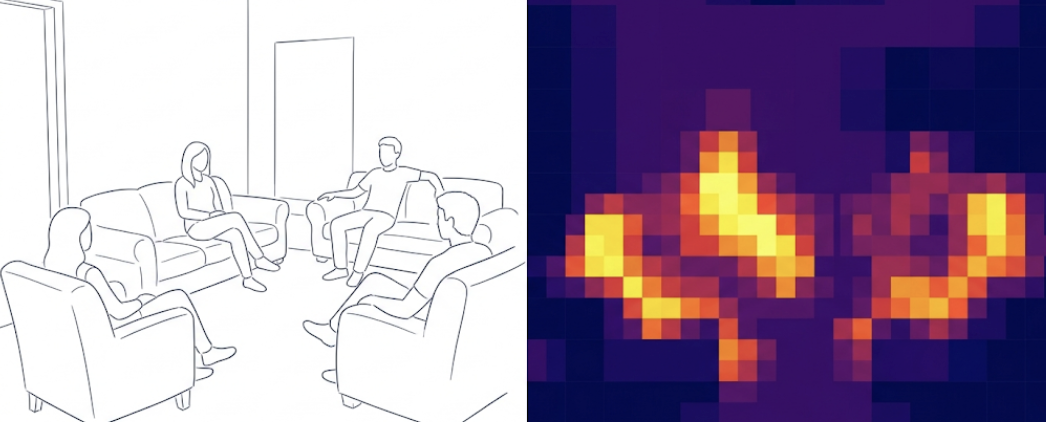
\includegraphics[width=0.75\textwidth]{r2photo.png}
    \caption{Koncepcyjny schemat topologii przestrzennej systemu. Skanowanie wnętrza za pomocą radaru (weryfikacja obecności statycznej) połączone z punktowym czytnikiem RFID w świetle drzwi.}
    \label{fig:topologia_sensorow}
\end{figure}

\subsection{Jak często "pytać" czujniki? (Twierdzenie Nyquista w praktyce)}
W tym miejscu pojawia się jednak pewien twardy problem fizyczny: jak często nasze radary ZigBee i czytniki powinny „pytać” pokój o to, co się w nim dzieje? Tutaj na białym koniu wjeżdża słynne twierdzenie Nyquista-Shannona z wykładów. Żeby nasz serwer nie zwariował od nadmiaru danych i żebyśmy poprawnie odwzorowali to, co faktycznie dzieje się w pokoju (czyli uniknęli tzw. aliasingu), musimy dobrać idealny interwał próbkowania. 

Gdybyśmy pobierali odczyt z radaru co 1 sekundę, zapchalibyśmy naszą sieć bezprzewodową gigantyczną ilością bezużytecznego szumu (nadmiarowość). Przecież studenci nie teleportują się z miejsc co sekundę! Z kolei sprawdzanie sali raz na 30 minut sprawi, że przegapimy momenty, kiedy ktoś wszedł, zjadł kanapkę i wyszedł. Z naszych pomiarów wynika, że średni czas rotacji na jednym krześle to około 15 minut. Dlatego na naszym serwerze na sztywno ustawiliśmy czas próbkowania (oznaczmy go jako $T_s$) na okrągłe 60 sekund. To w zupełności wystarczy, żeby wyłapać każdego nowego bywalca i świetnie odfiltrować szum (np. kogoś, kto tylko przeszedł przez pokój, żeby otworzyć okno).

\begin{figure}[H]
    \centering
    \begin{tikzpicture}
        \begin{axis}[
            width=0.85\textwidth,
            height=6.5cm,
            xlabel={Czas obserwacji pokoju [min]},
            ylabel={Liczba studentów},
            ymin=0, ymax=10,
            xmin=0, xmax=30,
            grid=both,
            minor tick num=1,
            legend style={
                at={(0.02,0.98)},
                anchor=north west,
                legend columns=1,
                fill=white,
                draw=black
            }
        ]
        % Ciągły sygnał rzeczywisty (Zjawisko)
        \addplot[smooth, thick, blue] coordinates {
            (0,2) (2,2) (4,5) (8,6) (12,6) (15,3) (20,3) (22,8) (26,8) (30,7)
        };
        \addlegendentry{Płynna rzeczywistość}
        
        % Dyskretne próbki (co 1 minutę - dla widoczności na wykresie co 2)
        \addplot[only marks, mark=square*, red, mark size=2pt] coordinates {
            (0,2) (2,2) (4,5) (6,6) (8,6) (10,6) (12,6) (14,4) (16,3) (18,3) (20,3) (22,8) (24,8) (26,8) (28,8) (30,7)
        };
        \addlegendentry{Nasze próbki z czujników ($T_s$)}
        \end{axis}
    \end{tikzpicture}
    \caption{Nasze podejście do próbkowania. Czerwone kwadraty pokazują momenty, w których system ściąga dane z sieci ZigBee, fajnie odzwierciedlając ciągłą rzeczywistość bez zapychania łącza.}
    \label{fig:probkowanie}
\end{figure}
\subsection{Poziom semantyczny: Interpretacja i sens informacji}

Aby odciążyć odbiorcę z nadmiarowości i dostarczyć wartość, dane muszą przejść cyfrową transformację na poziom semantyczny. Tu nasz autorski algorytm łączy i przetwarza surowe ciągi w konkretną wiedzę, dokonując dogłębnej interpretacji w pełni uwzględniającej anonimowość.

W naszym projekcie stawiamy na bardzo proste, programistyczne połączenie odczytów z obu urządzeń. Na poziomie semantycznym, zadaniem naszego oprogramowania jest po prostu zestawienie ze sobą surowych liczb i wywnioskowanie z nich jednego, pewnego wyniku dla konkretnej sali.

Działa to w naszej logice następująco: radar podwieszony nad małym pokojem do nauki (o pojemności 6 krzeseł) przesyła nam na serwer informację po API, że widzi fizycznie 4 osoby. Z kolei z bazy czytnika kart wynika, że wejście "odbiły" tylko 3 osoby. Nasz algorytm zawsze bezpiecznie wybiera większą wartość z tych dwóch źródeł, żeby się ubezpieczyć przed błędem sprzętowym (w tym przypadku zakładamy, że jeden student najzwyczajniej wszedł za kolegą bez przykładania własnej legitymacji do drzwi). Radar mądrze doliczył nam więc "brakującego" człowieka.

Mając wiarygodną wartość, system musi nadać jej jeszcze proste znaczenie (czyli przejść do warstwy semantycznej w 100\%). Skrypt analizuje, że skoro sala ma wpisany stały limit 6 wolnych miejsc, to oprogramowanie w mgnieniu oka redukuje całą tę skomplikowaną dedukcję do czytelnego, graficznego komunikatu. Na wielkim ekranie w lobby zapala się prosty napis: \textbf{,,Zajętość strefy: 4/6 miejsc''}.

Z perspektywy teorii i inżynierii danych określilibyśmy to klasycznym przeskokiem wymiarowości. Za kulisami ukrywamy zapytania do bazy języka SQL, wyliczany ruch milimetrowy Zigbee z opóźnieniami sieciowymi, a docelowo serwujemy studentowi na dole jasny wynik ułamkowy 4/6. Rzut oka na taki czysty kafel w systemie i nasz statystyczny odbiorca w sekundę podejmie decyzję, co robi dalej bez marnowania przerw między zajęciami na daremtne wycieczki po uczelni.

\subsection{Struktury wiedzy: Taksonomia stanów pokoju}

Żeby wyliczone obłożenie ułamkowe wyświetlało się w sensowny i szybki sposób dla studentów, ujednoliciliśmy podział stanów z progami z sekcji 2.3 i rozszerzyliśmy go o unikalny tryb techniczny. Aplikacja na serwerze przydziela je u dołu ekranów automatycznie, dając na mapie odpowiedni kolor kafelka:

\begin{enumerate}
    \item \textbf{WOLNE / DUŻO MIEJSC} \textcolor{green}{\textbf{(Zielony, 0-50\%):}} W sali dostępna jest wyraźna liczba wolnych miejsc. Status ten odpowiada pełnej lub wysokiej dostępności i zachęca do wejścia bez ryzyka ,,pustego przebiegu''.
    \item \textbf{UMIARKOWANY RUCH} \textcolor{yellow!60!black}{\textbf{(Żółty, 51-80\%):}} W pomieszczeniu trwa normalny ruch i nadal można znaleźć pojedyncze wolne miejsca, ale komfort wyboru jest mniejszy niż w strefie zielonej.
    \item \textbf{PRAWIE PEŁNY} \textcolor{orange}{\textbf{(Pomarańczowy, >80\% i <100\%):}} Poziom zajętości jest krytyczny. System zaczyna aktywnie promować alternatywne lokalizacje, aby ograniczyć niepotrzebne przejścia studentów.
    \item \textbf{PEŁNY} \textcolor{red}{\textbf{(Czerwony, 100\%):}} Brak wolnych miejsc siedzących. Sala jest oznaczana jako chwilowo niedostępna i pojawia się komunikat o rekomendowanej alternatywie.
    \item \textbf{SPRZĄTANIE} \textcolor{gray}{\textbf{(Szary, tryb techniczny):}} Mechanizm twardego serwisu o najwyższych uprawnieniach systemowych w hierarchii. Gdy pracownik techniczny odbija na czytniku swoją autoryzacyjną Kartę Master, nadpisuje to z automatu całą inteligentną detekcję danego pomieszczenia. Pokój znika z grafu operacyjnego dla całego wydziału aż do momentu ponownego zwolnienia karty po wyjściu obsługi.
\end{enumerate}

Podsumowując, nasz unikalny system podejmuje długą i solidną drogę programistyczną. Zaczynamy od hardware'owych detektorów pod sufitem ograniczających problematykę RODO (syntaktyka). Następnie zestawiamy je z wejściami legitymacji i wyliczamy ułamek zajętości miejsc, ubezpieczając się na wypadek wejścia kogoś niejawnie (semantyka). Wrzucenie tego w końcową, wielostopniową listę statusów stanowi dowód na to, jak z tysiąca odczytów radiowych uzyskać prostą i użyteczną tablicę decyzji dla zabieganego studenta przed wykładem.
\subsection{Ile faktycznie "wiedzy" daje system? (Entropia Shannona)}
Ale ile tak naprawdę czystej „wiedzy” dajemy studentowi na tym ekranie? Żeby nie być gołosłownym, postanowiliśmy przeliczyć to korzystając z matematycznego aparatu teorii informacji. Zgodnie z koncepcją Shannona, wartość informacji to po prostu „element zaskoczenia”. Im rzadszy jest dany kolor kafelka na ekranie, tym bardziej redukuje on naszą niepewność i tym więcej „bitów informacji” ze sobą niesie.

Zebraliśmy próbne statystyki z naszego radaru z najbardziej obleganych godzin (10:00 - 14:00) dla testowej sali Jet Brains. Wyszło nam, że pełny, 5-stanowy model rozkłada się następująco:
\begin{itemize}
    \item \textbf{Wolne / Dużo miejsc (Zielony):} 35\% czasu ($p = 0.35$).
    \item \textbf{Umiarkowany ruch (Żółty):} 30\% czasu ($p = 0.30$).
    \item \textbf{Prawie pełny (Pomarańczowy):} 20\% czasu ($p = 0.20$).
    \item \textbf{Pełny (Czerwony):} 10\% czasu ($p = 0.10$).
    \item \textbf{Sprzątanie (Szary):} 5\% czasu ($p = 0.05$).
\end{itemize}

Teraz wystarczy wrzucić to do klasycznego wzoru na samoinformację: $I(x) = -\log_2(p(x))$.
\begin{table}[H]
    \centering
    \renewcommand{\arraystretch}{1.3}
    \begin{tabular}{|l|c|c|}
        \hline
        \textbf{Kolor na ekranie} & \textbf{Prawdopodobieństwo} & \textbf{Ilość informacji [bit]} \\
        \hline
        Zielony (Wolne / Dużo miejsc) & $0.35$ & $\sim 1.51$ \\
        \hline
        Żółty (Umiarkowany ruch) & $0.30$ & $\sim 1.74$ \\
        \hline
        Pomarańczowy (Prawie pełny) & $0.20$ & $\sim 2.32$ \\
        \hline
        Czerwony (Pełny) & $0.10$ & $\sim 3.32$ \\
        \hline
        Szary (Sprzątanie) & $0.05$ & $\sim 4.32$ \\
        \hline
    \end{tabular}
    \caption{Twarde wyliczenie bitów informacji dla naszych kafelków.}
    \label{tab:entropia}
\end{table}

Jak na dłoni widać, że jak system wypluje szary kafelek „Sprzątanie”, to student dostaje gigantyczny strzał informacyjny (aż 4.32 bita zaskoczenia), bo to bardzo rzadka sytuacja. Z kolei zielony i żółty status pojawiają się częściej, więc niosą mniej informacji jednostkowej.

Mając te liczby, z łatwością policzyliśmy średnią niepewność (czyli słynną Entropię $H$) całego naszego wirtualnego pokoju:
\begin{equation}
    H(X) = \sum p(x) \cdot I(x) = (0.35 \cdot 1.51) + (0.30 \cdot 1.74) + (0.20 \cdot 2.32) + (0.10 \cdot 3.32) + (0.05 \cdot 4.32) \approx 2.06 \text{ bit/symbol}
\end{equation}

Maksymalna entropia dla układu 5-stanowego wynosi w teorii około $\log_2(5) \approx 2.32$ bita. Nasz wynik, czyli 2.06 bita na każde spojrzenie na ekran, to mocny dowód pragmatyczny. Pokazuje to czarno na białym, że nasza wizualizacja zdejmuje ze studentów konkretną porcję niewiadomych, optymalizując ich ruchy po wydziale.
\subsection{Architektura przesyłu danych}

Aby system tak płynnie przechodził od czujników do ostatecznej oceny zajętości na wyświetlaczach w holu, korzystamy ze świetnie zaplanowanej architektury technologicznej. Poniższy obraz przedstawia najważniejsze moduły tego układu:

\begin{figure}[h!]
    \centering
    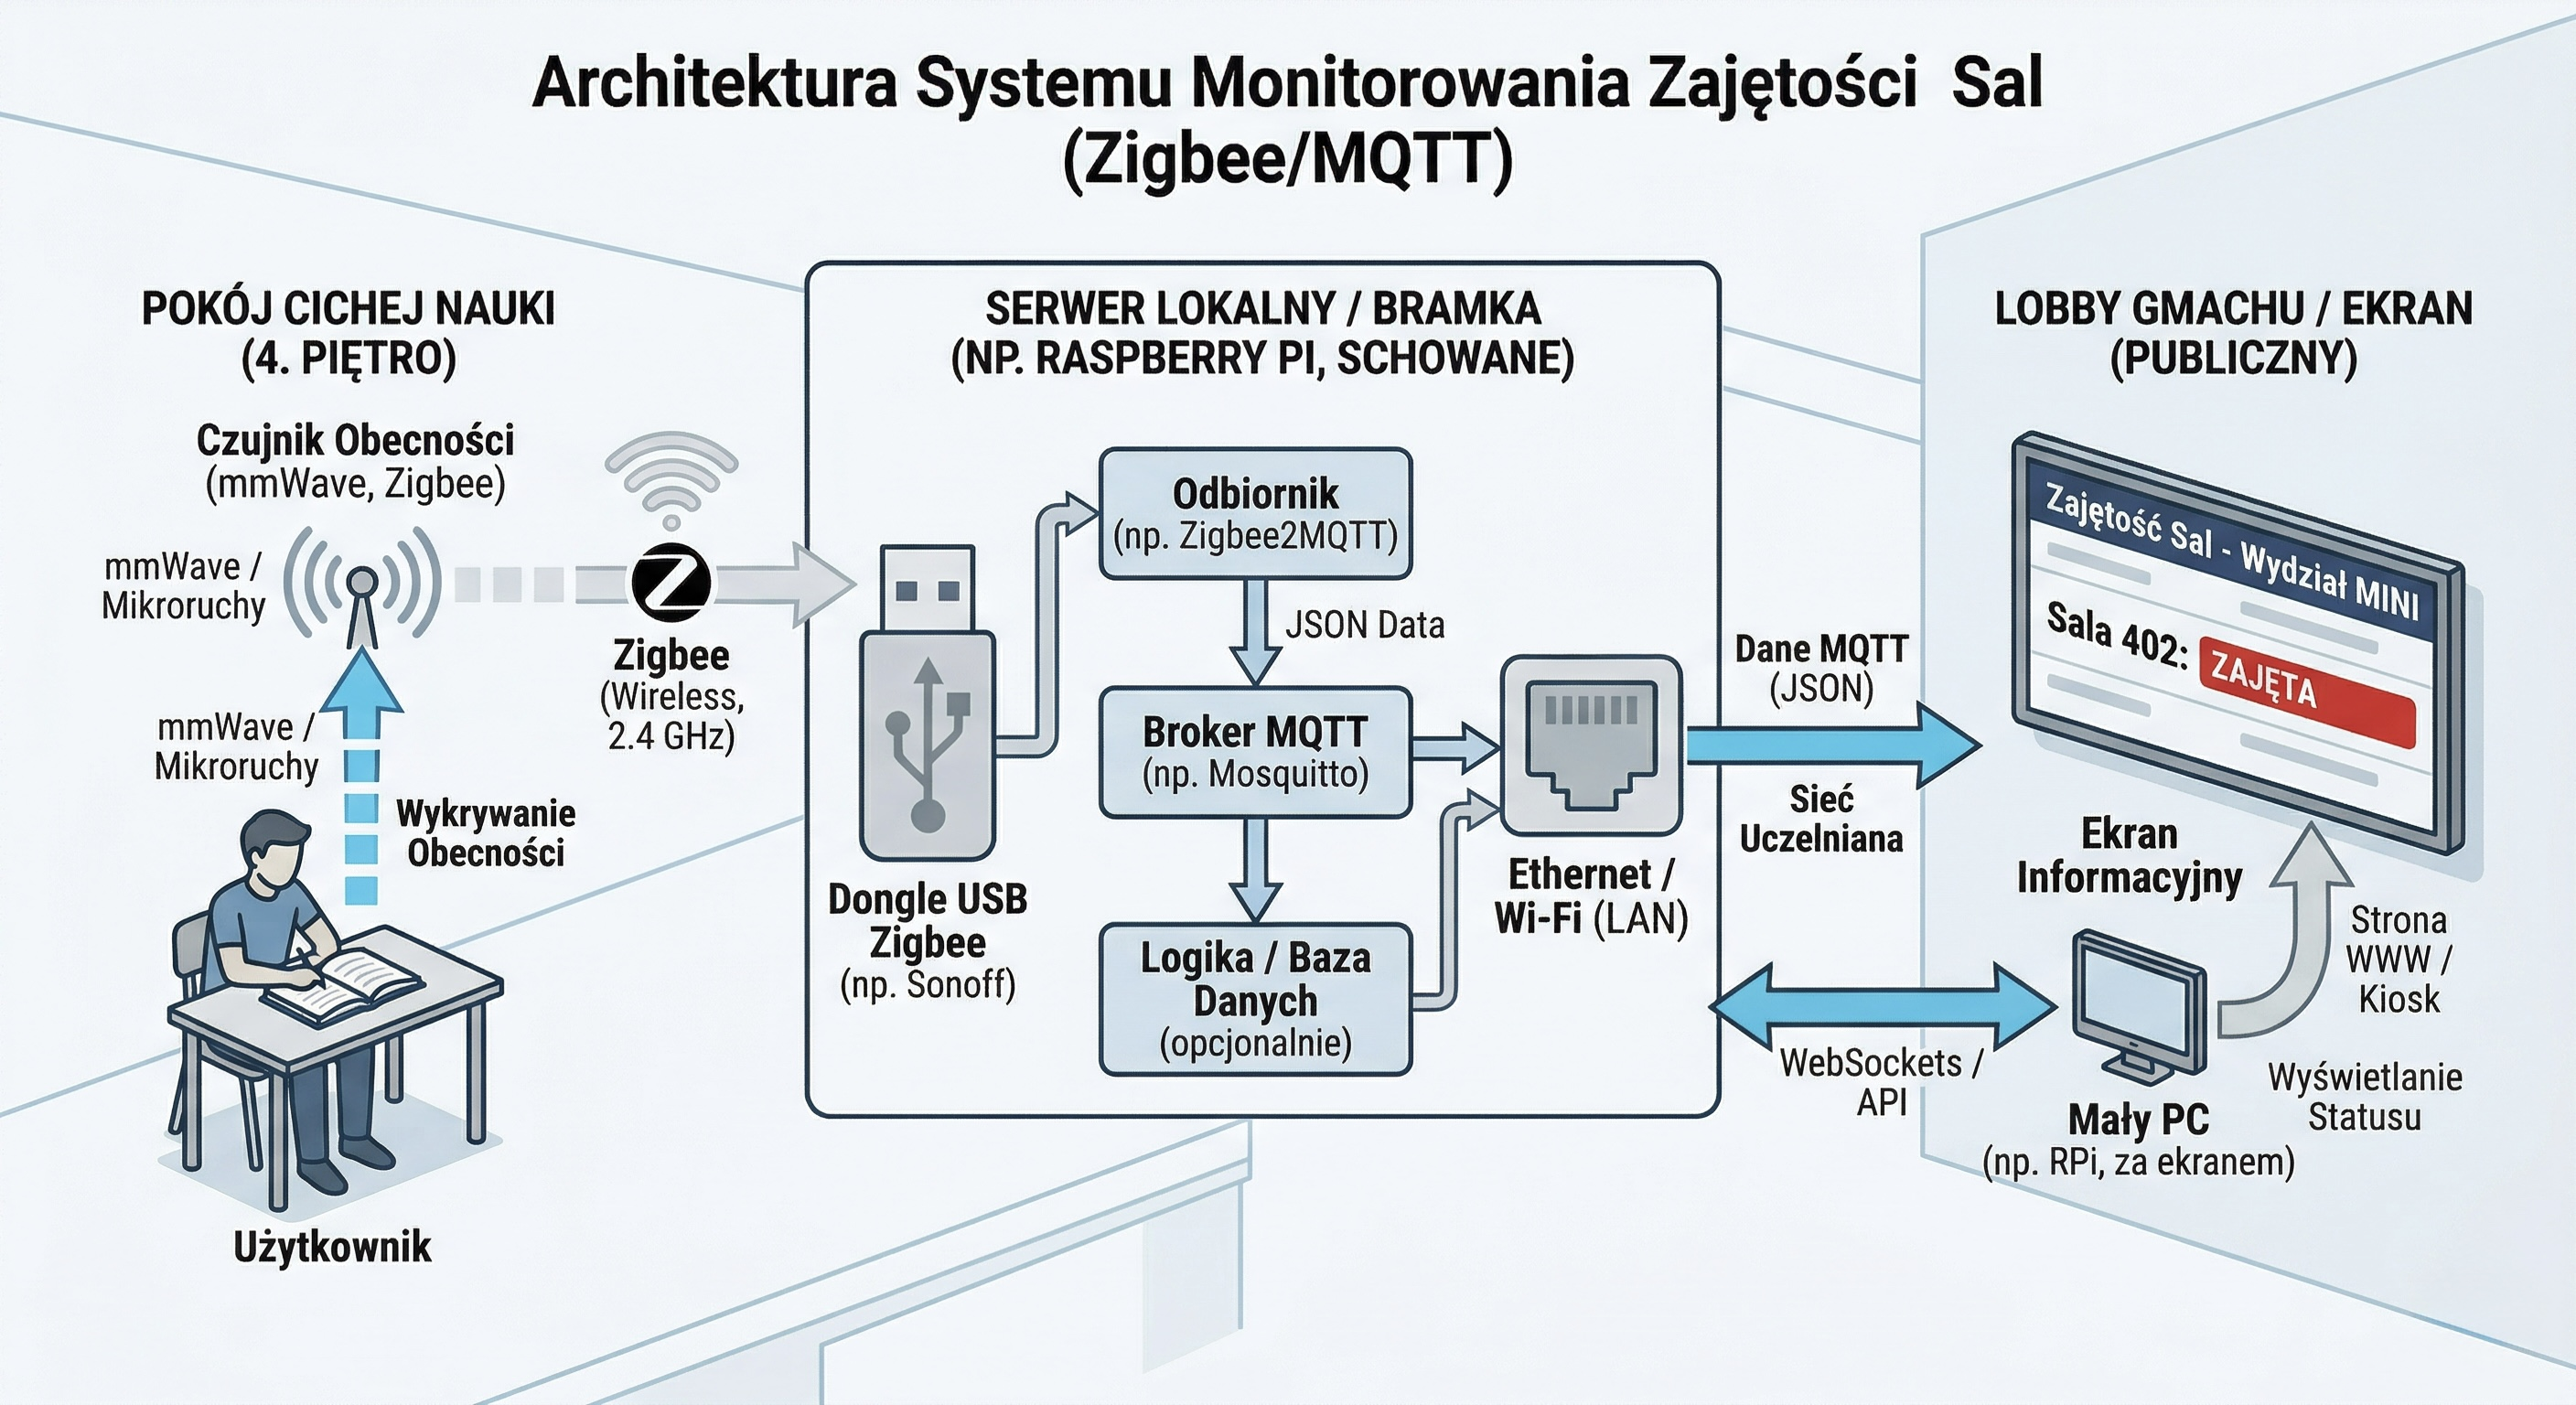
\includegraphics[width=\textwidth]{architektura.jpg}
    \caption{Architektura Systemu Monitorowania Zajętości Sal w technologii Zigbee i MQTT.}
    \label{fig:architektura}
\end{figure}

Działanie całości jest bardzo proste i można je opisać w zaledwie trzech krokach przepływu informacji:

\begin{itemize}
    \item \textbf{1. Środowisko fizyczne (Pokój Nauki - lewa strona):} Czujnik (rozpoznający ruch fizyczny z radaru) wykrywa, że student siedzi przy biurku. Ponieważ używa niezwykle energooszczędnej technologii Zigbee, wysyła wynik detekcji w powietrze drogą bezprzewodową na częstotliwości 2.4 GHz.
    \item \textbf{2. Hub Główny (Serwer Ukryty - środek):} Gdzieś dalej w budynku schowany jest malutki mikrokomputer nadzorczy (np. tanie, małe Raspberry Pi). Posiada on wetknięty do gniazda "gwizdek" USB (dongle przypominający pendrive), który świetnie radzi sobie z przechwytywaniem tych sygnałów z powietrza. Kiedy komputer je wyłapie, specjalne programy narzędziowe (np. protokół MQTT) tłumaczą surowy szum antenowy na klasyczny, ludzki tekst komputerowy typu "stan: obecność" i wgrywają to do głównej, twardej sieci ethernetowej uczelni.
    \item \textbf{3. Klient Końcowy (Z publicznym ekranem - prawa strona):} Sam wielki telewizor w holu wyposażony jest po prostu w kolejny minikomputer stykający się ze stroną WWW. Ten komputer w holu nie przeprowadza detekcji ani żadnych skomplikowanych obliczeń radarów i anten – jest stacją wyjściową. Przez internet co chwilę komunikuje się dyskretnie z Serwerem Ukrytym i na podstawie gotowego już wyniku po prostu maluje duży pasujący kafelek statusu ("Sala: Zajęta") prosto w oczy mijających go potoków studentów.
\end{itemize}

Rozbicie fizyki na te trzy elementy sprzętowe mocno upraszcza pisanie każdej linijki kodu oraz pozwala np. zresetować duży ekran w holu bez przerywania analizy liczenia wejściówek do stref nauki.

\end{document}
